\section{Results}
\label{sec:results}

\subsection{Impulsive Aggression}
\label{sub:impulsive_aggression_gwas}

No significant hits were identified in $\sim37,320$ subjects (see Figure~\ref{fig:gwas_impAgg}).
This is unfortunate but not surprising giving the low number of individuals.

\begin{figure}[!h]
  \begin{subfigure}{.5\textwidth}
    \centering
    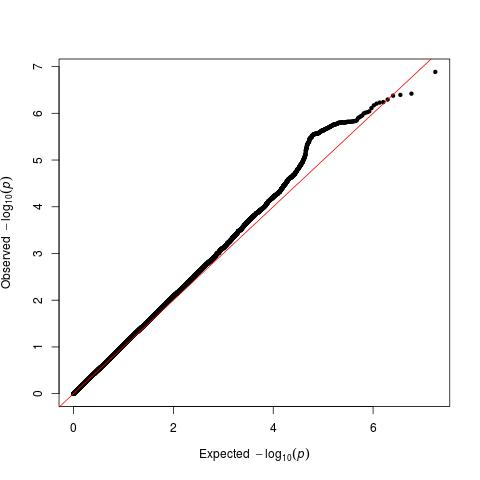
\includegraphics[width=0.8\linewidth]{{assoc_results/post_gwas/qq_plots/qq_plot_4526}.jpeg}
    \caption{QQ-plot for Impulsive aggression}\label{fig:ImpAgqq}
  \end{subfigure}
  \begin{subfigure}{.5\textwidth}
    \centering
    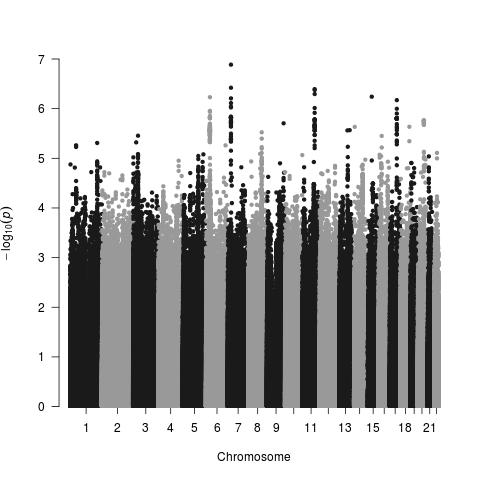
\includegraphics[width=0.8\linewidth]{{assoc_results/post_gwas/manhatten_plots/manhatten_plot_4526}.jpeg}
    \caption{Manhattan plot for Impulsive aggression}\label{fig:ImpAgmanhatten}
  \end{subfigure}
  \caption{GWAS on Impulsive aggression\label{fig:gwas_impAgg}}
\end{figure}

While no population stratification has been identified (Table~\ref{tab:LDscImpAgg}) SNP heritability is relatively low.

\begin{table}[!htpb]
	\centering
	\caption{LDsc results for Impulsive aggression}
	\label{tab:LDscImpAgg}
	%latex.default(out, file = paste0(outputfolder, "ldscore_results_",     variable_name, ".tex"), table.env = F, rowname = NULL)%
\begin{center}
\begin{tabular}{llll}
\hline\hline
\multicolumn{1}{c}{Total Observed scale h2}&\multicolumn{1}{c}{Lambda GC}&\multicolumn{1}{c}{Intercept}&\multicolumn{1}{c}{Ratio}\tabularnewline
\hline
0.0532 (0.012)&1.0496&1.0082 (0.0056)&0.1693 (0.1163)\tabularnewline
\hline
\end{tabular}\end{center}

\end{table}

\subsection{Risk Taking}
\label{sub:risk_taking_gwas}

Next I performed a GWAS on risk taking.
As of \today, I was unable to find any study looking at this phenotype within the UKB\@.
Due to the large sample size, in contrast to the previous described results (see section~\ref{ssub:impulsive_aggression_gwas}), I will evaluate the results in more detail (since I actually have some).
Risk taking is coded according to table~\ref{tab:coding} thus it has the same coding as impulsive aggression.
In total there were $120,286$ subjects available with a complete phenotype.
The corresponding QQ and Manhattan plot are displayed in figure~\ref{fig:risktaking_gwas}, and the lead SNPs are shown in table~\ref{tab:lead_snps_risk}.
As mentioned above, lead SNPs were identified using clumping.
LD-score regression indicates no major population stratification since both intercept and ratio approaches $0$ (see table~\ref{tab:ldscrisk}).

As you can see in the Manhattan plot in figure~\ref{fig:riskmanhatten} there are two clear signal in chromosome 3 and 6, as well as a signal which is just below genome wide significant at chromosome 4.
A closer inspection of the signal in chromosome 3 shows 2 lead SNPs (see table~\ref{tab:lead_snps_risk}).
However, \textit{rs1308431} and \textit{rs7639518} have opposite directions of effect.
In order to investigate if the signals are independent of each other I performed a conditional analysis.
Using the top SNP (\textit{rs13084531}) as a covariate, the analysis showed no independent genome-wide significant effect.
Thus suggesting that \textit{rs7639518} is not independent of \textit{rs13084531}.
However, a closer look at the conditional regression model suggest that the \textit{rs7639518} might be a potentially independent signal (see table~\ref{tab:conditional}) since the resulting p-value is relatively low. 
I will need to see if an increase in statistical power might result in two separate signals within this area in the next stage of the UKB.
Unfortunately, an internal replication within the UKB was not successful (see section~\ref{ssub:Replication}).

\begin{figure}[!h]
	\caption{GWAS on Risk Taking}
	\label{fig:risktaking_gwas}
	\begin{subfigure}{.5\textwidth}
		\centering
		\caption{QQ-Plot of risk taking}
		\label{fig:riskqq}
		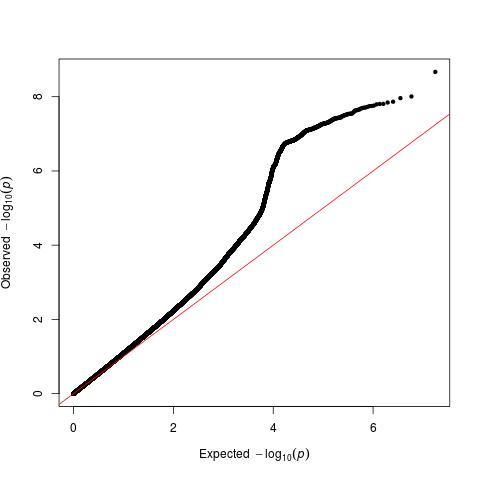
\includegraphics[width=0.8\linewidth]{{assoc_results/post_gwas/qq_plots/qq_plot_2040}.jpeg}
	\end{subfigure}
	\begin{subfigure}{.5\textwidth}
		\centering
		\caption{Manhattan plot of risk taking}
		\label{fig:riskmanhatten}
		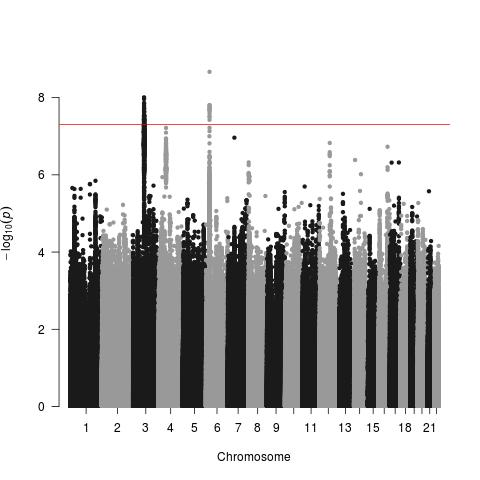
\includegraphics[width=0.8\linewidth]{{assoc_results/post_gwas/manhatten_plots/manhatten_plot_2040}.jpeg}
	\end{subfigure}
\end{figure}

Below I will describe the three identified regions of interest (the two genome wide significant signals as well as the one approaching significance).
I also performed a quick literature review as well as looked up the three SNPs in the GWAS catalog (see table~\ref{tab:gwas_risk_catalog})

\paragraph{rs9379971}
\label{par:rs9379971}
This particular variant has the strongest association among all tested SNPs with a p-value of $2.14e-09$. 
The SNP is an intronic variant, without any mentioning in the GWAS catalog \citep{Welter2014}.
As you can see in the LocusZoom plot (figure~\ref{fig:rs9379971}) the region round the identified SNPs is rather dense. 
The SNPs has been associated with \textit{POM121L2} and the region has been connected with schizophrenia across multiple studies \citep{Aberg2013,Shi2009}.
However, the function of \textit{POM121L2} is not well understood.

\paragraph{rs13084531}
\label{par:rs13084531}
As you can see in figure~\ref{fig:rs13084531} the variant is in a relatively large LD region with a comparable p-value to the previous SNP ($9.826e-09$).
The SNPs is an intron variant within the gene \textit{CADM2}.
The gene has been associated with BMI \citep{Speliotes2010} as well as executive functions and processing speed \citep{Ibrahim-Verbaas2015}.
Interestingly the SNP associated in the study by \cite{Ibrahim-Verbaas2015} (rs17518584) is in LD to our loci (rs13084531 with $R^2=0.4951;D'=0.9983$).
Hence suggesting a common loci for executive functions and risk taking.
Further the region of this SNP (3p12.1) has been connected to spirometric measures in smokers \citep{Lutz2015}.

\paragraph{rs4386663}
\label{par:rs4386663}
This SNP is an intergenic variant with no known association with any regulatory functions.
However, the SNP is only marginal significant ($6.059e-08$).
Interestingly, however, the chromosomal region of this SNP (chr4q12) was also associated with spirometric measures in smokers by the same study as in variant rs13084531 (see paragraph~\ref{par:rs13084531}.
The LocusZoom plot (see figure~\ref{fig:rs13084531}) suggests a relatively narrow LD region. 

\begin{table}
	\small
	\centering
	\caption{Lead SNPs reaching genome wide significance in Risk Taking}\label{tab:lead_snps_risk}
	%latex.default(dat, title = "", file = paste0(outputfolder, "lead_snp_",     nameID, ".tex"), digits = 3, rowname = NULL, table.env = F)%
\begin{center}
\begin{tabular}{rlrlrrrr}
\hline\hline
\multicolumn{1}{c}{CHR}&\multicolumn{1}{c}{SNP}&\multicolumn{1}{c}{BP}&\multicolumn{1}{c}{A1}&\multicolumn{1}{c}{NMISS}&\multicolumn{1}{c}{OR}&\multicolumn{1}{c}{STAT}&\multicolumn{1}{c}{P}\tabularnewline
\hline
$3$&rs76395182&$85547337$&T&$108695$&$1.063$&$ 5.72$&$1.09e-08$\tabularnewline
$3$&rs13084531&$85553994$&C&$115264$&$0.936$&$-5.73$&$9.83e-09$\tabularnewline
$6$&rs9379971&$27259308$&T&$109344$&$1.065$&$ 5.99$&$2.14e-09$\tabularnewline
\hline
\end{tabular}\end{center}

\end{table}

\begin{table}[!htpb]
	\centering
	\caption{Additional SNP catalog look up for Risk Taking}\label{tab:gwas_risk_catalog}
	\resizebox{\textwidth}{!}{%latex.default(dat, title = "", file = paste0(outputfolder, "gwas_catalog_",     nameID, ".tex"), digits = 3, rowname = NULL, table.env = F)%
\begin{tabular}{lrlrlrl}
\hline\hline
\multicolumn{1}{c}{Lead SNP}&\multicolumn{1}{c}{P}&\multicolumn{1}{c}{Study SNP}&\multicolumn{1}{c}{Study P}&\multicolumn{1}{c}{Disease Trait}&\multicolumn{1}{c}{PubMedID}&\multicolumn{1}{c}{Direction}\tabularnewline
\hline
rs13084531&$9.83e-09$&rs9841144&$9e-07$&Longevity (90 years and older)&$25199915$&yes\tabularnewline
rs13084531&$9.83e-09$&rs13323436&$3e-06$&Visceral fat&$22589738$&\tabularnewline
rs9379971&$2.14e-09$&rs16897515&$4e-07$&Schizophrenia&$23894747$&no\tabularnewline
rs9379971&$2.14e-09$&rs6932590&$1e-12$&Schizophrenia&$19571808$&yes\tabularnewline
\hline
\end{tabular}
}
\end{table}

\begin{table}[!htpb]
	\small
	\centering
	\caption{Risk Taking with \textit{rs13084531} as covariate for selected SNP}
	\label{tab:conditional}
	\resizebox{\textwidth}{!}{%latex.default(dat, title = "", file = "conditional_analysis_rs13084531.tex",     table.env = F, col.names = F)%
\begin{tabular}{lrlrlrrrr}
\hline\hline
\multicolumn{1}{l}{}&\multicolumn{1}{c}{CHR}&\multicolumn{1}{c}{SNP}&\multicolumn{1}{c}{BP}&\multicolumn{1}{c}{A1}&\multicolumn{1}{c}{NMISS}&\multicolumn{1}{c}{OR}&\multicolumn{1}{c}{STAT}&\multicolumn{1}{c}{P}\tabularnewline
\hline
2&$3$&rs76395182&$85547337$&G&$107738$&$0.957$&$-3.787$&$0.0001523$\tabularnewline
\hline
\end{tabular}
}
\end{table}

\begin{table}[!htpb]
	\centering
	\caption{LDsc results for risk taking}
	\label{tab:ldscrisk}
	%latex.default(out, file = paste0(outputfolder, "ldscore_results_",     variable_name, ".tex"), table.env = F, rowname = NULL)%
\begin{center}
\begin{tabular}{llll}
\hline\hline
\multicolumn{1}{c}{Total Observed scale h2}&\multicolumn{1}{c}{Lambda GC}&\multicolumn{1}{c}{Intercept}&\multicolumn{1}{c}{Ratio}\tabularnewline
\hline
0.0552 (0.0052)&1.127&1.0056 (0.0069)&0.0422 (0.052)\tabularnewline
\hline
\end{tabular}\end{center}

\end{table}

